% #############################################################################
% This is Appendix Model Integrations
% !TEX root = main.tex
% #############################################################################
\chapter{Model Integrations}
\label{chap:app004}

This appendix delves into the integration of \ac{DL} models in the clinical workflow of breast cancer diagnosis, focusing on the design of intelligent agents.
Leveraging advanced \ac{DL} models and integrating them into medical imaging systems holds tremendous potential for enhancing the accuracy and efficiency of breast cancer diagnosis (Section~\ref{sec:chap003003} of Chapter~\ref{chap:chap003}).
The goal of this appendix is to provide a comprehensive analysis of various \ac{DL} models specifically tailored for medical imaging tasks related to breast cancer diagnosis (Section~\ref{sec:chap002005} of Chapter~\ref{chap:chap002}).
Through this exploration, we aim to shed light on the strengths and limitations of these models, considering their architectural innovations and application potential.
Understanding the intricacies of these models allows us to identify opportunities, leading to more effective outcomes for the developments under this thesis.

The latter part of the appendix details the process of pre-processing medical imaging data and integrating these models into a real-world clinical setting.
Emphasis is placed on the importance of data normalization, model training, and the crucial steps involved in deploying these models into a clinical setting.
Furthermore, this appendix provides insights into the strategies for improving system performance and resolving potential issues during the testing phase.
This appendix is a foundation for understanding the technical aspects that underpin the successful application of \ac{ML} methods in medical imaging.

\section{Deep Learning Methods Overview}
\label{sec:app004001}

Medical images are hard to classify and segment because their anatomical structures (Section~\ref{sec:chap002004} of Chapter~\ref{chap:chap002}) vary in shape and size~\cite{10.1007/978-3-030-00934-2_99}.
The representational power and capacity for capturing structural information of \acp{CNN}, have made such classification (Section~\ref{sec:app004001001}) and segmentation (Section~\ref{sec:app004001002}) possible~\cite{Hou_2016_CVPR}.
The literature shows that the detection of lesions in breast cancer is highly inconsistent~\cite{shen2019deep}.
Breast cancer detection methods can be divided into five main approaches:
(i) traditional image acquisition techniques;
(ii) image enhancement model, especially for noise removal;
(iii) finding cancer-affected areas by detecting the suspicious \ac{ROI} on medical images while using suitable segmentation method;
(iv) feature extraction, such as {\it radiomics}; and
(v) classification of normal, benign, or malign from \ac{ROI}.
Making it vital to create a proper model pipeline (Figure~\ref{fig:fig027}) to achieve better segmentation, feature extraction, and classification.

%%%%%%%%%%%%%%%%%%%%%%%%%%%%%%%%%%%%%%%%%%%%%%%%%%%
\begin{figure}[htbp]
\centering
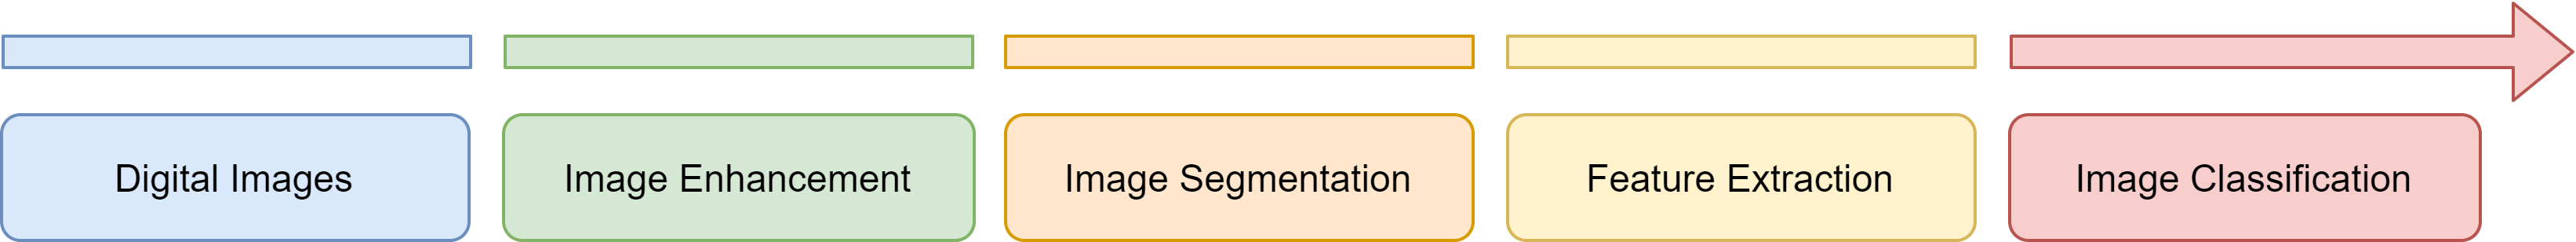
\includegraphics[width=\columnwidth]{images/fig027}
\caption{A simple diagram for the proposed model pipeline of breast cancer detection. First, digital images are acquired. Second, image enhancement must proceed. Third, computing image segmentation. Fourth, extraction of features. The fifth and final is the classification of images.}
\label{fig:fig027}
\end{figure}
%%%%%%%%%%%%%%%%%%%%%%%%%%%%%%%%%%%%%%%%%%%%%%%%%%%

Numerous studies~\cite{wang2018support, milosevic2017comparison} discuss various methods for early breast cancer detection.
This thesis addresses such works, with some methods already implemented and others planned for future integration.
A classification model has been combined with an intelligent agent and evaluated by clinicians (see Chapter~\ref{chap:chap005} and Chapter~\ref{chap:chap006}).
While the integration of a segmentation model is underway, it has not yet been completed due to clinicians' prioritization of the \ac{BI-RADS} classification information.
Thus, it will be addressed further in future work (Chapter~\ref{chap:chap008}).

Although several works~\cite{9247957} are arguing to follow a specific pipeline (Figure~\ref{fig:fig027}), it is not mandatory for staying strict to that order, like other authors did~\cite{8451510, AGRAWAL201927}.
During the development and integration of these methods, the order of each process can be changed without losing model accuracy~\cite{8462671}.
This thesis is focused on the introduction of intelligent agents as a \ac{HCI} perspective, instead of optimizing the model accuracy.
Therefore, jumping to the final stage of the pipeline (Figure~\ref{fig:fig027}), and starting from the end, will be fair to cover the main concerns of this thesis.

Regarding the above pipeline order ({\it i.e.}, segmentation, feature extraction, and classification), each process can be fulfilled separately~\cite{8451510, AGRAWAL201927} and brought together~\cite{10.1007/978-3-030-00934-2_99} at the end of the thesis.
For a proper patient diagnostic, the final classification is the most critical task.
Specifically, the use case achieved from an automatic classification (\ac{BI-RADS}) is the process in which clinicians are informed of the final diagnostic results.
That said, a use case for patient classification is of chief importance for the clinicians' workflow.

In this thesis, the segmentation will support the process of making an intelligent agent more explainable (\ac{XAI}) and interpretable~\cite{8622433}.
For instance, the segmentation can inform the clinician where the lesions are and why ({\it e.g.}, with colors and heatmaps) is the \ac{BI-RADS} so high.
However, segmentation models are more challenging to train~\cite{TAJBAKHSH2020101693}.
Due to a lack of available data~\cite{ahmed2020images}, segmentation models are hard to implement accurately compared to classification models for the medical imaging domain~\cite{murtaza2019deep}.
One crucial fact is that image-level labels (weak annotations)~\cite{10.1145/3373017.3373051}, cumming from the classification process, are easier to get for the training set~\cite{TAJBAKHSH2020101693}.
To train a model, the segmentation process is more time-consuming, and manual lesion annotations are harder to get from clinicians~\cite{10.1007/978-3-030-59719-1_44}.
Hence, the work under this thesis started first by developing intelligent agents to inform clinicians about patient classification.

\subsection{Classification Outline}
\label{sec:app004001001}

From the literature, recently proposed \ac{DenseNet}~\cite{Huang_2017_CVPR} is one of the most used \ac{CNN} structures for the classification of lesions in medical imaging~\cite{LIU2019e271}.
The model connects all the preceding layers as the input for a particular layer, which can strengthen feature propagation ({\it e.g.}, {\it radiomics}) and alleviate the gradient vanishing problem~\cite{10.1145/3136755.3143016}.
Furthermore, due to the feature reuse, the \ac{DenseNet} model only needs to learn a small set of new features in each layer.
Thus, the model requires fewer parameters than traditional \acp{CNN}, which is more suitable for small datasets, such as the one created under this thesis.
In this thesis work, a multimodality \ac{DenseNet} model was integrated to solve the classification problem.
The task is to classify inputs of \ac{MG} (both in \ac{CC} and \ac{MLO}), \ac{US}, and \ac{MRI} images.
Along with \ac{GT} of masses and microcalcifications, the masks of the model can classify (either normal, benign, or malign) into the correct class.

\subsection{Segmentation Outline}
\label{sec:app004001002}

The above section describes several literary works and challenges this thesis must address to integrate classification and segmentation models into intelligent agents for a proper medical imaging diagnosis.
In this section, the document focuses on the works~\cite{Dabbous397} that will promote and motivate the future integration of segmentation models.
Specifically, one motivation for that integration will be to provide clinicians the visualization of lesions, making these models infer their decisions~\cite{CHOUGRAD201819, doi:10.1148/radiol.2018181371}.
Additionally, these detected lesions can be further applied to aid the training of \acp{DNN}~\cite{8032490, 8861376}.
In this thesis, a multimodality HyperDenseNet~\cite{8515234} model is proposed to be integrated and to solve the segmentation problem.
The task will be to segment inputs of breast images into binary lesion masks, such as masses and microcalcifications.
However, these are just future thoughts being out of the scope of this document, which describes the work achieved until now.

\section{Published Datasets Preview}
\label{sec:app004002}

In breast screening, published research results are difficult to replicate due to the lack of datasets in the area of \acp{CDSSe}~\cite{lee2017curated}.
Most of the used classification (Section~\ref{sec:app004001001}) and segmentation (Section~\ref{sec:app004001002}) methods are evaluated on private datasets or on unspecified subsets of public databases.
These methods are integrated as algorithms for a proper \ac{CADe} and \ac{CADx} on breast cancer and are designed to assist clinicians in a better diagnostic interpretation.
Despite promising results, current \ac{CADe} systems are limited by high \ac{FP} rates, and \ac{CADx} systems for breast screening are not yet approved for clinical use because of the lack of available data~\cite{10.1145/3079765}.

Few well-curated public datasets and databases have been provided for the research community.
These include INbreast, \ac{MIAS} and the most recent \ac{DDSM}~\cite{shen2019deep}.
Although these public datasets are helpful, they are limited in data accessibility, completeness, and size.
Moreover, datasets are limited in terms of single-modality images ({\it i.e.}, on \ac{MG}-only information) and do not provide any co-variables\footnotemark[28] of the patients.
Such information is so crucial to clinicians' workflow.
Furthermore, most researchers use these datasets without leveraging their images for various reasons~\cite{lee2017curated}.
For instance, the \ac{ROI} annotations for the abnormalities in \ac{DDSM} were provided to indicate a general position of lesions, but not a precise segmentation and classification for them.
Therefore, in this thesis, it was also developed a tool (Chapter~\ref{chap:chap004}) that generates a novel dataset jointly with clinicians.
This feature covers the implementation problem and limitations of algorithms for accurate feature extraction.

%%%%%%%%%%%%%%%%%%%%%%%%%%%%%%%%%%%%%%%%%%%%%%%%%%%
\footnotetext[28]{The hazard of patient diagnosis must be modeled as a function of several co-variables, such as pathological results, age, morbidity, patient behaviors ({\it e.g.}, smoking), and tumor history, among others. Current datasets do not contain any information about these co-variables. A prognostic model that predicts the final diagnostic result and aids in primary clinicians' decision-making must consider these co-variables for early breast cancer detection.}
%%%%%%%%%%%%%%%%%%%%%%%%%%%%%%%%%%%%%%%%%%%%%%%%%%%

\section{Neural Network Integration}
\label{sec:app004003}

In this section, we provide additional details concerning using the DenseNet integrated into our \ac{UI}.
This process not only involved mere implementation, but also required significant optimization to align with our objectives.
Concretely, we provide additional details concerning the following:
(i) the dataset;
(ii) data pre-processing;
(iii) evaluation strategy;
(iv) learning methodology;
(v) transfer learning; and
(vi) additional description of the system.
We aim to present a clear and extensive understanding of our procedures, shedding light on the technical underpinnings that contribute to the robustness and effectiveness of our approach.
This in-depth explanation will provide a thorough perspective on our methodology, supporting its replication and further improvements.

\subsection{Comparison with Existing Methodologies}
\label{sec:app004003001}

Regarding model comparison with existing methods, the literature shows improvements in the DenseNet model concerning mean sensitivity and specificity by surpassing, for example, the EfficientNet model~\cite{jpm10040211}.
For instance, the authors report the Mean \ac{AUC} for detecting breast cancer was 0.952~\textpm~0.005 by a DenseNet model and 0.954~\textpm~0.020 by an EfficientNet model.
Moreover, the authors further report the mean sensitivity and specificity from a DenseNet model, of 87\% and 88\%, respectively, surpassed the mean values, of 81\% and 82\%, obtained in their meta-analysis.
Hence, the literature has demonstrated the DenseNet model efficiency~\cite{8633197, Hai2019}.

\subsection{Dataset Size}
\label{sec:app004003002}

In this work, we used 338 cases acquired in the \acf{HFF}.
From this set of cases, 289 were classified by the head of the radiology department from the \ac{HFF} clinical institution.
Each patient has several images concerning four  X-ray \acs{MG} (two \acs{CC} views for \acs{CC} left and \acs{CC} right, as well as two \acs{MLO} views for \acs{MLO} left and \acs{MLO} right), one \acs{US} image, and roughly five images in \acs{MRI}.
In the \ac{MRI} volumes, we take several image slices per patient, where the lesion is present (recall point 5) in the previous question).
This provides us roughly 2890 images ({\it i.e.}, 289~\texttimes~(4 + 1 + 5)), that are used to train/test the \ac{DL} model (DenseNet).
Although we tried to balance the number of patients between \acs{BI-RADS} scores, our dataset only has 11\% of \acs{BI-RADS} = 3.
Therefore, reducing the generalizability power of the \ac{DL} model for these cases.

\subsection{Data Pre-Processing}
\label{sec:app004003003}

Traditional image processing and deep learning techniques require extensive pre-processing.
It is known that a cleaning dataset is welcome when training a deep neural network~\cite{RIASATIAN2021102032}.
In our study, this stage is of the utmost importance, since the \ac{MG}, \ac{US}, and \ac{MRI} images contain quite different intensities and sizes.
Thus, before introducing the images to the DenseNet, we pre-process the data.
Specifically, we perform a data normalization, so that the images have the same intensity, regardless of the modality.

All images used in our system are resized to a resolution of 224x224 pixels, ensuring uniformity in the input data structure for DenseNet and reducing computational demands.
Furthermore, we normalize each image's pixel intensity by subtracting the mean and dividing by the standard deviation.
This process harmonizes variations in illumination and contrasts across images, facilitating more efficient learning by keeping inputs within a similar range.
These pre-processing steps are vital not only because DenseNet is designed to accept this specific input format, but also streamline the learning process, enhancing model performance and yielding more consistent results.

\subsection{DenseNet Steps}
\label{sec:app004003004}

\vspace{2.50mm}

\noindent
The DenseNet steps are as follows:

\vspace{0.50mm}

\begin{enumerate}

\item The DenseNet is pre-trained with the ImageNet model that contains roughly 1.2 million images. This gives generalization capabilities to new datasets.

\vspace{0.50mm}

\item Next, we remove the last layer of the DenseNet (that contains numerous classes, about 1000 classes or end-nodes) and replace it with a fully connected layer containing now three nodes.
Each node of the network corresponds to one of the following classes:
(i) low severity (Class 1: BIRADS $<=$ 1),
(ii) medium severity  (Class 2:  1 $<$ BIRADS $<=$ 3), and
(iii) high severity (Class 3: BIRADS $>$ 3).
Thus, we have a DenseNet with three nodes in the last layer.

\vspace{0.50mm}

\item Now, the pre-trained DenseNet goes through a process of fine-tuning in our breast dataset.
The dataset comprises 1125 training images ({\it i.e.}, \ac{MG} in both \ac{CC} and \ac{MLO} views, \ac{US}, and \ac{MRI}). Notice that here, we have 338 cases or patients (Section~\ref{sec:chap005005003} of Chapter~\ref{chap:chap005}).
The more significant number of training images, when compared to the number of patients, stems from the fact that one patient may have more than one image.

\vspace{0.50mm}

\item We split the above dataset in the following way: 80\% for training and the remaining 20\% for testing.
In this partition, we guarantee that each set (training and test) is properly balanced, that is, each set contains samples that belong to all classes (recall that there are three classes as mentioned in Section~\ref{sec:chap005005003} of Chapter~\ref{chap:chap005}), see also point 1) and all modalities ({\it i.e.}, \ac{MG}, \ac{US}, and \ac{MRI}).
Therefore, the experiments take into consideration multimodality.

\vspace{0.50mm}

\item The pre-training follows a supervised learning strategy.
Specifically, during the training we provide the image, as well as the corresponding label, that is, the classification in one of the three classes for the image.
This classification ({\it i.e.}, \ac{GT}) is provided by a set of eight radiologists (Section~\ref{sec:chap005005} of Chapter~\ref{chap:chap005})).
Say that this training stage gives the DenseNet the ability to establish associations between the morphology of the lesion (image) and its severity (classification label).

\vspace{0.50mm}

\item Finally, we use the held-out test set to measure the performance of the DenseNet.
An accuracy of 98.2\% was obtained in this test set.

\vspace{0.50mm}

\item As a final note, we should mention that the three patients (as mentioned in Section~\ref{sec:chap005005001} of Chapter~\ref{chap:chap005})) are obtained from the test set as mentioned above (see point 4).
From the above, the number of test samples is high.
However, only three samples are taken  for the experiment's purpose.
Thus, the training and testing phases take into account numerous samples.

\end{enumerate}

\section{Training and Evaluation of the DenseNet}
\label{sec:app004004}

The evaluation mechanism for the DenseNet follows a two-stage process, involving training and testing stages.
To accomplish this, we partition the dataset (Section~\ref{sec:app004003002}) to form the training and testing subsets in the following manner:
80\% of the samples are used for training, and the remaining 20\% for testing.
In this partition, we guarantee that each set (training and test) is appropriately balanced.
That is, each set contains samples that belong to all five and in all modalities ({\it i.e.}, \ac{MG}, \ac{US}, and \ac{MRI}) - this is to guarantee  the multimodality.

\vspace{1mm}

\noindent
{\it Training}:
The training follows a supervised learning strategy.
Specifically, during the training, we provide the image, as well as the corresponding label, that is, the classification \ac{BI-RADS} score.
The head of radiology of the \ac{HFF} institution provides this classification ({\it i.e.}, \ac{GT}, between the real and the predicted results).
This allows the DenseNet ability to establish associations between the morphology of the lesion (image) and its severity (classification label).

\vspace{1mm}

\noindent
{\it Testing}:
During the test phase, we used a hold-out test set that aimed to measure  the performance of the DenseNet.
An accuracy of 94.81\% was obtained in this test set. 
Notice that the three patients (as mentioned in Section~\ref{sec:chap005005003} of Chapter~\ref{chap:chap005}) are obtained from this hold-out test set.

\vspace{2mm}

\noindent
{\it Remark}: 
Another possibility for DenseNet training is to resort to unsupervised learning  methods.
However, this class of approaches is more challenging, since only the images are fed into the network without the help of having the classification labels ({\it i.e.}, without \ac{BI-RADS} classification in training).
This deserves our attention in future work.

\section{Transfer Learning}
\label{sec:app004005}

As a final remark, we should stress that although the  number of samples is relatively small (less than 3000 images, as mentioned in Section~\ref{sec:app004003002}), we may argue that this could be not enough since a robust training \acp{DNN} usually require large amounts of annotated samples (order of 100Ks) to avoid overfitting to the training data given the large model capacity.
This issue can be handled with the so-called ``\acl{TL}'' (\acs{TL}).
Basically, the \acs{TL} process retrains (in a process called fine-tuning) publicly available models (pre-trained with large datasets) using smaller datasets.

Utilizing a DenseNet model pre-trained on the expansive ImageNet dataset, with over 1.2 million diverse images, enabled us to initialize our network and speed up the convergence of our deep architecture~\cite{8515234}.
The DenseNet structure is particularly effective in mammogram classification due to its feature reuse capabilities, as highlighted in two pivotal works~\cite{10.1007/978-3-030-88163-4_16, 10.1007/978-3-030-47679-3_23}.
This method not only accelerates the learning process, but also enhances the model's generalization performance in the specific context of breast cancer detection.

It has been demonstrated that this \ac{TL} approach is possible to be applied in the medical image field, even if the datasets used in this pre-training stage are completely different from the medical images - in this case - different from breast images~\cite{8032490}.
This is precisely what we did here.
Concretely, we used a pre-trained that provides the \ac{DNN} more regularization and generalization capabilities to new datasets.
In the experiments, the DenseNet was pre-trained with the ImageNet model that contains millions of images from 1000 classes (Section~\ref{sec:app004003004}).
The only adjustment required  to adapt the DenseNet is to change the last layer from 1000 nodes (or classes) to the number of five classes (Section~\ref{sec:app005009} of Appendix~\ref{chap:app005}) in our problem.

\section{DenseNet Final Remarks}
\label{sec:app004006}

The DenseNet is a complex model.
This means that the model can handle heterogeneous types of input.
Thus, given the relatively small number of training samples, it is advantageous to join all the modalities.

\vspace{2.50mm}

\noindent
In the experiments, we have compared two situations:

\vspace{1.50mm}

\begin{enumerate}
\item Joining all the modalities to a single DenseNet; and
\item Using three different DenseNet, each network for each image modality type (\ac{MG}, \ac{US}, and \ac{MRI}).
\end{enumerate}

\vspace{1.50mm}

\noindent
{\bf Note:} the best results were achieved for situation (1), and this was adopted for our \ac{UI}.

\section{Additional Description of the System}
\label{sec:app004007}

\vspace{1.50mm}

\noindent
Now we detail a little better the description of the system, as follows:

\begin{enumerate}
\item Each of the 289 patients was classified by the head of radiology of the Medical Imaging Department at the \ac{HFF} institution.
This classification corresponds to assigning a \ac{BI-RADS} value for each modality image of the exam;
\item We trained our DenseNet across the \ac{BI-RADS}, (we already detailed how the  training/test of the DenseNet is accomplished);
\item After the training, we have the test phase.
Here the new (unseen) images are presented to the DenseNet, and a \ac{BI-RADS} classification is provided to that test sample; and
\item To evaluate the system's accuracy, the precision, and recall are computed.
\end{enumerate}

% \vspace{2mm}

\noindent
The following link is available that illustrates eases the description of the proposed system, as well as its workflow:

\vspace{2mm}

\noindent
\href{https://youtu.be/k2vBpbKqJqQ}{youtu.be/k2vBpbKqJqQ}

%%%%%%%%%%%%%%%%%%%%%%%%%%%%%%%%%%%%%%%%%%%%%%%%%%%
\begin{figure}[htbp]
\centering
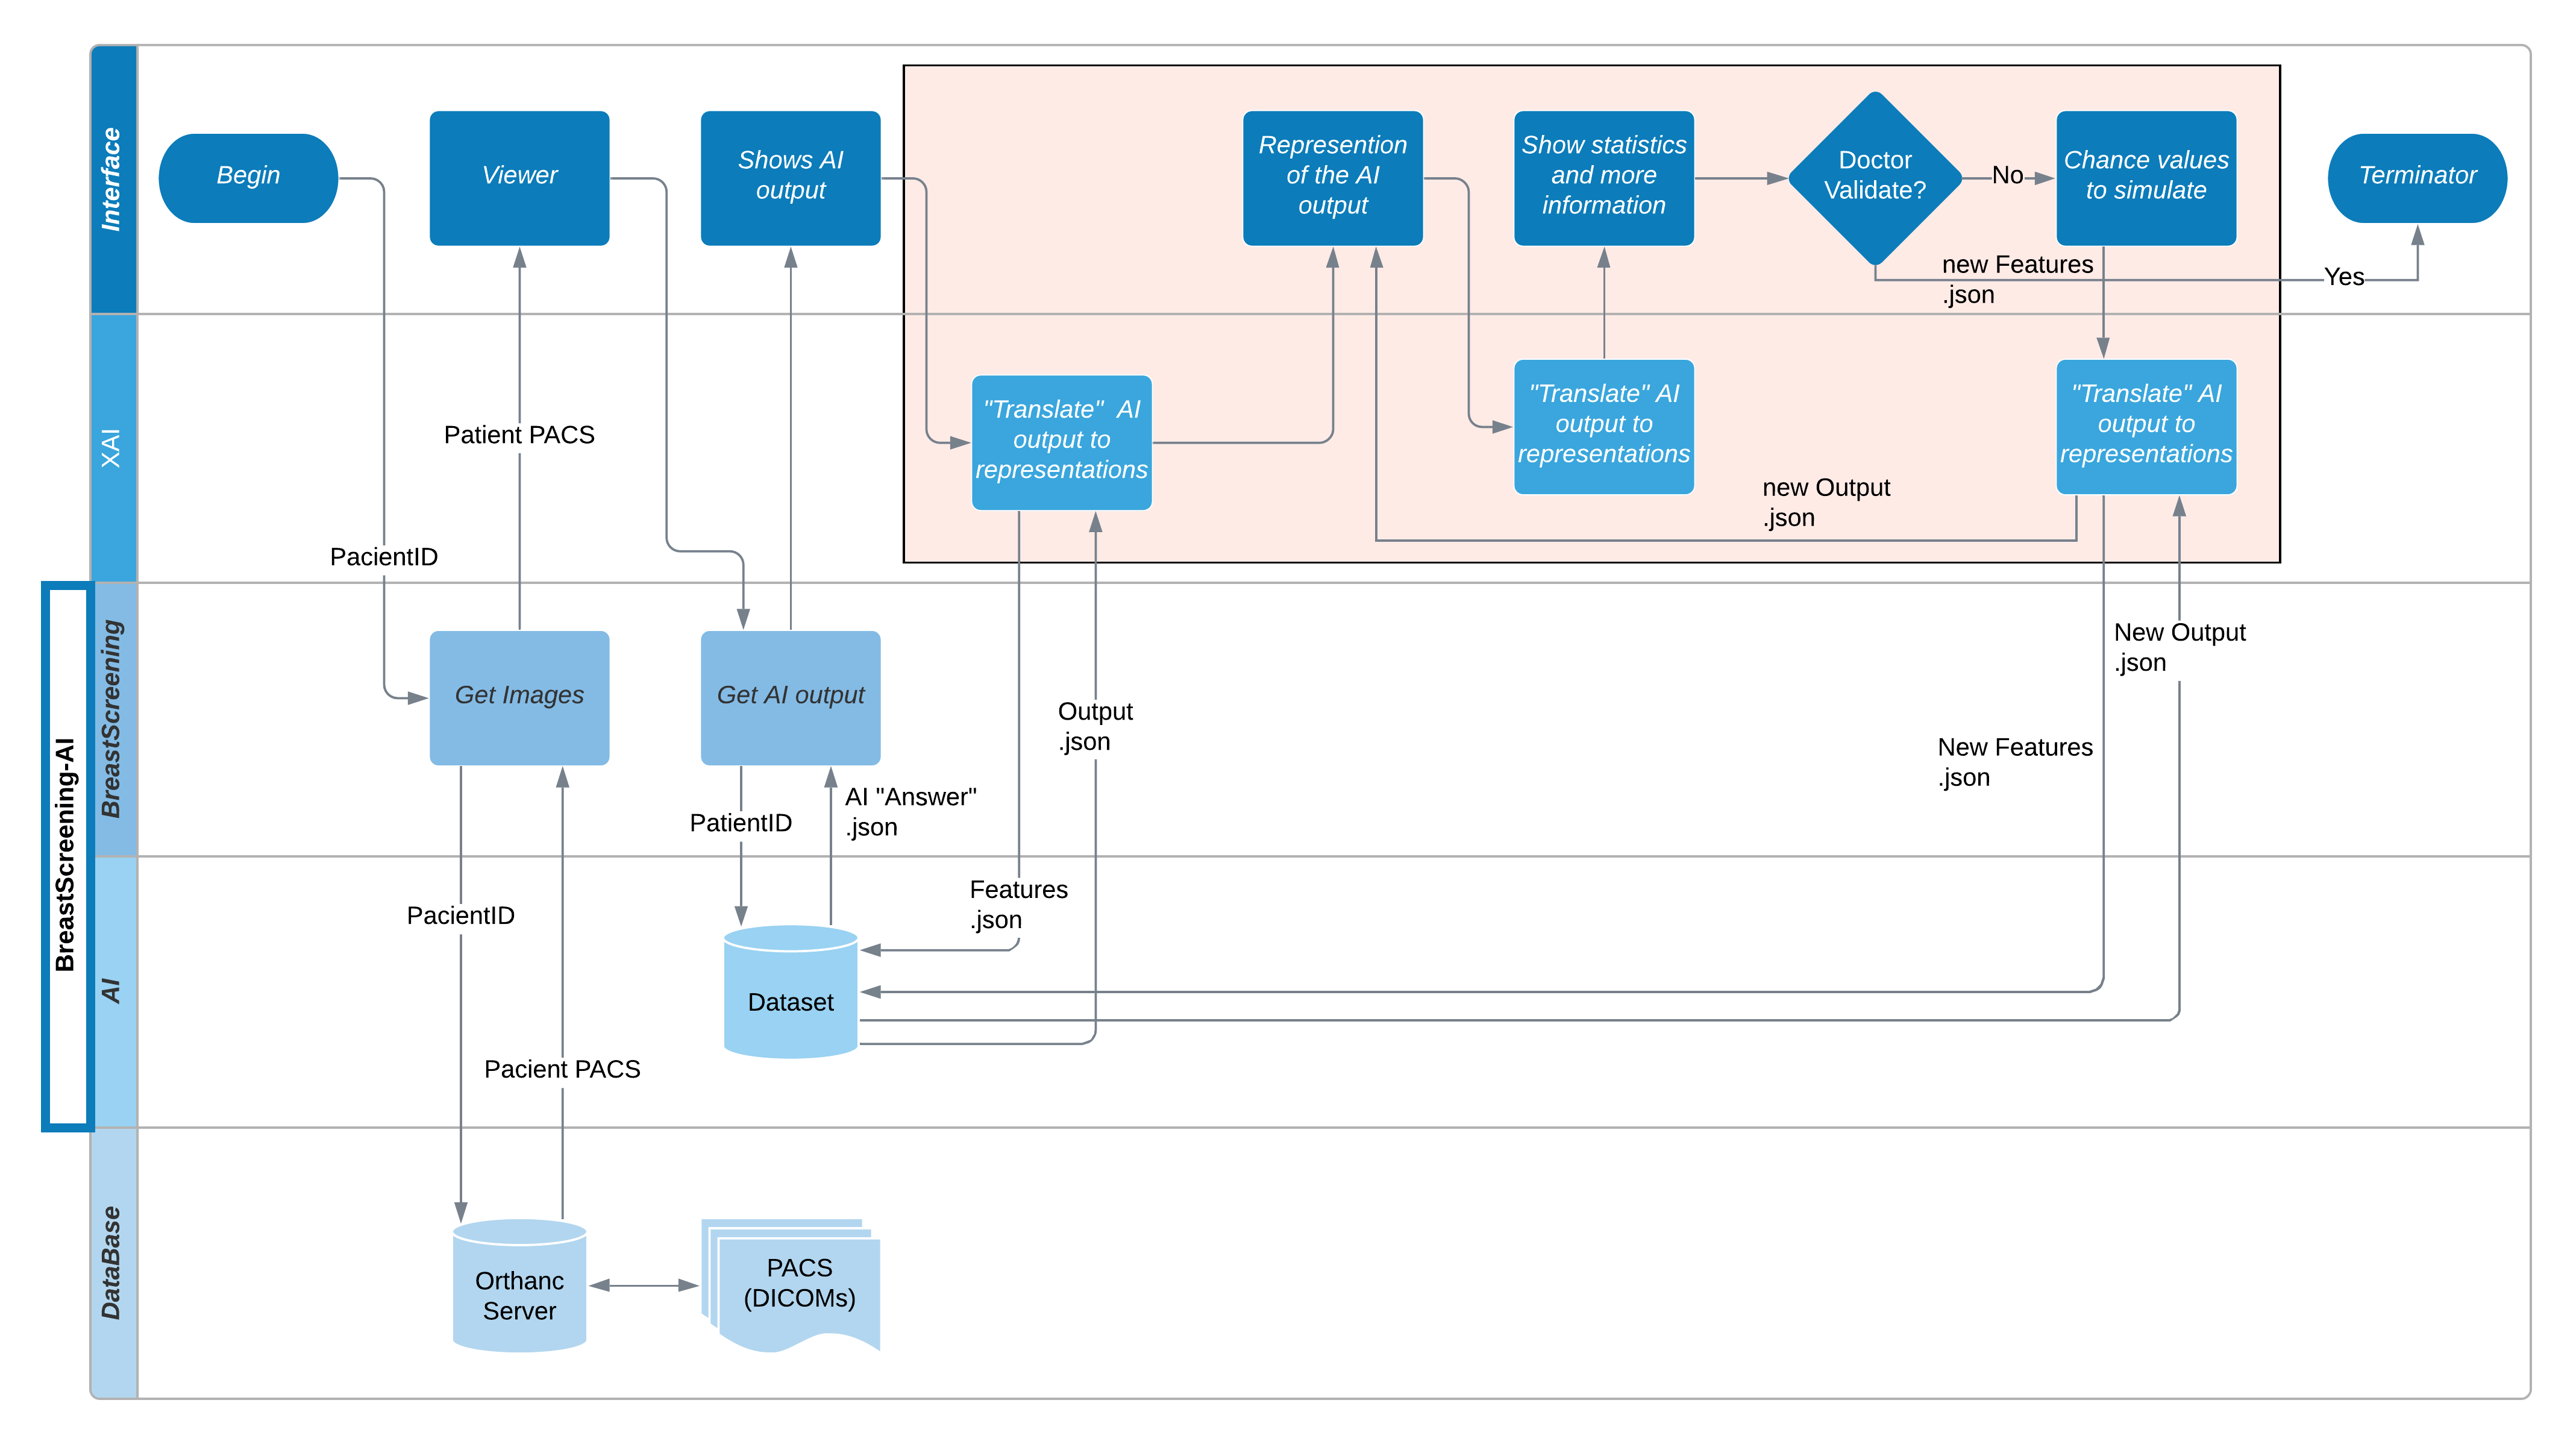
\includegraphics[width=0.925\textwidth]{fig072}
\caption{Architecture and functionalities diagram of the typical use cases. These use cases are presented with the order of actions for the interrogated AI system.}
\label{fig:fig072}
\end{figure}
%%%%%%%%%%%%%%%%%%%%%%%%%%%%%%%%%%%%%%%%%%%%%%%%%%%

\section{Separate vs. All Modalities}
\label{sec:app004008}

As illustrated in Table~\ref{tab:tab016}, the performance noticeably elevates when operating in a multimodal context compared to the unimodal.
This enhancement is primarily due to the significant expansion of the training dataset, encompassing all imaging modalities.
Consequently, the model benefits from a larger pool of images with a broader range of variability.
This data augmentation serves a dual purpose -- it bolsters the regularization of the DenseNet model while simultaneously curbing overfitting, thereby leading to superior generalization capabilities.
In the unimodal case, the lack of an extensive training dataset resulted in severe over-fitting issues, despite our efforts to mitigate this through:
(i) data augmentation strategies, where each image is randomly modified in each batch using common transformations, such as small rotations, flipping, and translations; and
(ii) other regularization strategies like dropout and L2 (weight decay).

Finally, we stress that the network architecture receives 2D images.
Since the \ac{DCE-MRI} are volumes, we extract some of the slices that contain the lesion.
All the above issues led the network to obtain significantly better results in the multimodal scenario, as demonstrated in Table~\ref{tab:tab016}.

\section{System Diagram}
\label{sec:app004009}

Concerning the system diagram of the BreastScreening-AI framework (Figure~\ref{fig:fig072}), the first action is to request the patients (Section~\ref{sec:chap002008} of Chapter~\ref{chap:chap002}) stored on the Orthanc server~\cite{Jodogne2018}.
Next, the assistant will show the \ac{AI} outputs.
Finally, clinicians can decide by accepting or rejecting the \ac{AI} suggestion (Section~\ref{sec:chap005004001} of Chapter~\ref{chap:chap005}).

As stated before (Section~\ref{sec:chap005004} of Chapter~\ref{chap:chap005}), our interface (Figure~\ref{fig:fig040}) has three main button functionalities ({\it i.e.}, 6.1. Accept; 6.2. Explain; and 6.3. Reject).
Each button of our interface generates different triggers on the framework (Figure~\ref{fig:fig072}).
Hence, three triggers are essential to denote (Appendix~\ref{chap:app008}).

%%%%%%%%%%%%%%%%%%%%%%%%%%%%%%%%%%%%%%%%%%%%%%%%%%%
\begin{table}[htpb]
\centering
\resizebox{\linewidth}{!}{%
\begin{tabular}{|c|cccc|c|}
\hline
Strategy   & \multicolumn{4}{c|}{Unimodal}                                                                  & \multirow{2}{*}{Multimodal} \\ \cline{1-5}
Modalities & \multicolumn{1}{c|}{CC-MG} & \multicolumn{1}{c|}{MLO-MG} & \multicolumn{1}{c|}{US}   & DCE-MRI &                             \\ \hline
Accuracy   & \multicolumn{1}{c|}{0.73}  & \multicolumn{1}{c|}{0.68}   & \multicolumn{1}{c|}{0.65} & 0.667   & 0.9481                      \\ \hline
\end{tabular}%
}
\caption{Evaluation results of the AI-Only for the unimodal tests with the DenseNet-121 model. Compared Models as unimodal training: Cranio-Caudal MG (CC-MG); Medio-Lateral Oblique MG (MLO-MG); UltraSound (US); and Dynamic Contrast-Enhanced MRI (DCE-MRI). Finaly, the multimodal training stands for CC-MG, MLO-MG, US, and DCE-MRI all modalities together.}
\label{tab:tab006}
\end{table}
%%%%%%%%%%%%%%%%%%%%%%%%%%%%%%%%%%%%%%%%%%%%%%%%%%%

The first trigger is made by clinicians when pressing the accept button, where a \ac{JSON} file is generated to provide success information to the model.
The second trigger represents the \ac{AI} model explanations.
Clinicians press the explain button, in order to have more reliable information concerning what regions were considered by the model and how severe these lesions are to the model.
Finally, the third trigger happens when clinicians reject the \ac{AI} result.
At this point, clinicians must provide the new \ac{BI-RADS} so that we can further retrain the \ac{AI} model.
To this end, the framework will generate a \ac{JSON} file with clinicians' new rejected \ac{BI-RADS} values.

\section{Conclusive Integrations}
\label{sec:app004010}

To conclude, this appendix offers an in-depth investigation across the integration of \ac{DL} models into the clinical workflow during breast cancer diagnosis (Section~\ref{sec:app004003}), focusing on developing intelligent agents.
Elucidating the subtle details of these models and the associated processes of pre-processing medical imaging data (Section~\ref{sec:chap006005002} of Chapter~\ref{chap:chap006}) for real-world clinical use paves the way to spotlight opportunities for the developments under this thesis.
Gaining insight into the strengths, limitations, and essential steps required for model deployment establishes a solid foundation for improving system performance and tackling potential issues that may arise during the testing phase.
Above all, this appendix is a thorough guide for employing \ac{ML} methods in medical imaging, highlighting their potential to refine the accuracy and efficiency between clinical humans and \ac{AI} systems.